\documentclass{article}
\usepackage{graphicx}
\usepackage{subfig}
\usepackage{indentfirst}
\usepackage{amsmath}

% Title Page
\title{MAE 5730 Final Project \\
\large{Dynamic modeling of a spy zip-lining into a objective}}
\author{Mark Lohatepanont}


\begin{document}
\maketitle
\newpage

\section{Project Specification}
My project is to model the dynamics of a human taking a zipline through a arbitrarily defined course. The human, or “spy” in the context of this document consists of a 3-link body connected to a point mass. The point mass is representative of the zipline trolley, and the 3 links represent the head-neck connection, neck-waist connection and then waist to toe connection. \\

        
\begin{figure}[h]
    \centering
	\subfloat[\centering Anatomical Body]{{\includegraphics[width=5cm]{2anatomical_model} }}%
	\qquad
	\subfloat[\centering Sledge]{{\includegraphics[width=5cm]{point_mass} }}%
	\caption{Description of model components}%
	\label{fig:example}%
\end{figure}

A description of the 3 link connection is established visually above in Figure 1a where each of the links are described as rigid bodies which have their own lengths, masses, moments of inertia as well as their rotation as defined from the perpendicular of the previous link. For some more anatomical accuracy, the body’s joints will also act as torque dampers. 
This body’s head is then connected to a point mass which serves as the trolley and the forcing of the system that drives the spy through the course. 
Figure 2b describes the point mass setup with the first link (head connection) also being shown. As mentioned, the point mass has a forcing which will drive it through the course.
The course itself will be described by 3 distinct functions (subject to change) and is described visually in figure 3.

\begin{figure}[h]
	\centering
	\includegraphics[scale=0.5]{course_description}	
	\caption{Description of course}
\end{figure}

The spy’s trolley will be attached to the lines shown and follow the course. Where the start is at X = 0, and the end at X = 15. (Subject to Change)
The goal of the project is to develop the model and a visual representation of the system that can be plotted. An additional goal would be to find out how much forcing can be applied to the spy’s trolley to 
get them to the end of the course as quick as possible before the links loop upon themselves which will metaphorically mean that the spy has died and unsuccessfully made it to the end. 

\section{Equations of Motion}
\subsection{Euler-Lagrange Method}
\subsubsection{Constraints}
The setup consists of one force leading to a non-conservative force, one holonomic constraint coming from the course, and one non-holonomic constraint coming from the torque dampers. I will deal with the holonomic constraint by using a Lagrange multiplier.  An example of how I deal with the trivial case of in the course where $y=-\frac{1}{10}x+16$, the holonomic constraint becomes $\dot{y}=\frac{1}{10}\dot{x}$, with the differential form being $fdt=dy-\frac{dx}{10}=0$, which leads to the Lagrange multipliers of $f_x=1$,$f_y=1$. These can then be incorporated into the equations of motion calculations.  For the torque damper, I’ll use the Raleigh dissipation equation to reduce the torque on the joints. Different sections of the course will be piece wised together. \\
For each of the three stages of the course using a holonomic constraint the differential form as well as the constraint is described in the following table:
\begin{center}
\begin{tabular}{c|c|c}
	Function&Differential Form&Constraint\\
	\hline
	$(\frac{x}{10}-3)^2+1$&$dy-\frac{\left(\frac{x}{10} - 3\right)}{5} dx=0$&$\ddot{y}=\frac{\dot{x}^2}{50} + \frac{\left(\frac{x}{10} - 3\right) \ddot{x}}{5}$\\
	$\frac{-1}{10}+16$&$dy+\frac{1}{10}dx$&$\ddot{y}=\frac{-1}{10}\ddot{x}$\\
	$-(\frac{x}{10}-12)^2+10$&$dy+\frac{\frac{x}{10}-12}{5}dx=0$&$\ddot{y}=-\frac{\dot{x}^2}{50}-\frac{\frac{x}{10}-12}{5}\ddot{x}$\\
\end{tabular}
\end{center}
\subsubsection{Lagrange Equations}
The generalized coordinates are chosen as the minimal set of coordinates $q_i = \{ x,y,\theta_1,\theta_2,\theta_3 \} $. The Lagrange equations come from the kinetic and potential energy. The kinetic energy can be found by summing up the kinetic energy of the sledge and each of the links combined with the rotational energy of each of the links. This is loosely described below in equation 1.
\begin{equation}\label{Kinetic Energy Equation}
	E_k = \frac{1}{2} \left( m_1 v_1^2 + m_2 v_2^2 + I_{g1} \dot{\theta}_1^2 + m_3 v_3^2 + I_{g2} \dot{\theta}_2^2 + m_4 v_4^2 + I_{g3} \dot{\theta}_3^2 \right) 
\end{equation}
The velocities $v1, v2, v3,$ and $v4$ can be found in the generalized coordinates by the following equations described in 2.:
\begin{equation}
	\begin{split}
		v_1 = \sqrt{\dot{x}_g^2 + \dot{y}_g^2} \\
		v_2 = \sqrt{\left( \dot{x}_g + d_1 \dot{\theta}_1 \cos(\theta_1) \right)^2 + \left( \dot{y}_g - d_1 \dot{\theta}_1 \sin(\theta_1) \right)^2} \\
		v_3 = \sqrt{\left( \dot{x}_g + d_1 \dot{\theta}_1 \cos(\theta_1) + d_2 \dot{\theta}_2 \cos(\theta_2) \right)^2 + \left( \dot{y}_g - d_1 \dot{\theta}_1 \sin(\theta_1) - d_2 \dot{\theta}_2 \sin(\theta_2) \right)^2}\\		
		v_4 = (\left( \dot{x}_g + d_1 \dot{\theta}_1 \cos(\theta_1) + d_2 \dot{\theta}_2 \cos(\theta_2) + d_3 \dot{\theta}_3 \cos(\theta_3) \right)^2 \\
		\quad + \left( \dot{y}_g - d_1 \dot{\theta}_1 \sin(\theta_1) - d_2 \dot{\theta}_2 \sin(\theta_2) - d_3 \dot{\theta}_3 \sin(\theta_3) \right)^2)^{0.5}
	\end{split}
\end{equation}
Finally, the potential energy is defined in 3 as the heights of the center of gravity of the point mass and each link measured from the datum where $y=0$:
\begin{equation}
	\begin{split}
			E_p = g ( m_1 y_g + m_2 \left( y_g - d_1 \cos(\theta_1) \right) + m_3 \left( y_g - d_1 \cos(\theta_1) - d_2 \cos(\theta_2) \right) \\
		+ m_4 \left( y_g - d_1 \cos(\theta_1) - d_2 \cos(\theta_2) - d_3 \cos(\theta_3) \right) )	
	\end{split}
\end{equation}
\newpage
\subsection{Differential Algebraic System of Equations Method (DAE)}
\subsubsection{Free Body Diagrams}
To aid in the DAE method, I created free body diagrams for each of the bodies in my system. The bodies are the sledge, shown in Figure 3a, link 1, shwon in figure 3b, link 2 shown in figure 3c, and link 3 shown in figure 3d. Using these free body diagrams, I generated 11 Newton-Euler equations by performing Linear Momentum Balance (LMB) on the sledge, link 1, link 2 and link 3 in both the $\hat{i}$ and $\hat{j}$ coordinate frames along with 3 angular momentum balance (AMB) around link 1, link 2 and link 3. Along with these equations I also generated 8 constraint equations, 6 coming the constraints in the $\hat{i}$ and $\hat{j}$ in each of the three links. The last two constraints come from the holonomic constraints for the normal force which comes from the sledge interacting with the course.
\begin{figure}[h]
	\centering
	\subfloat[\centering Sledge FBD]{{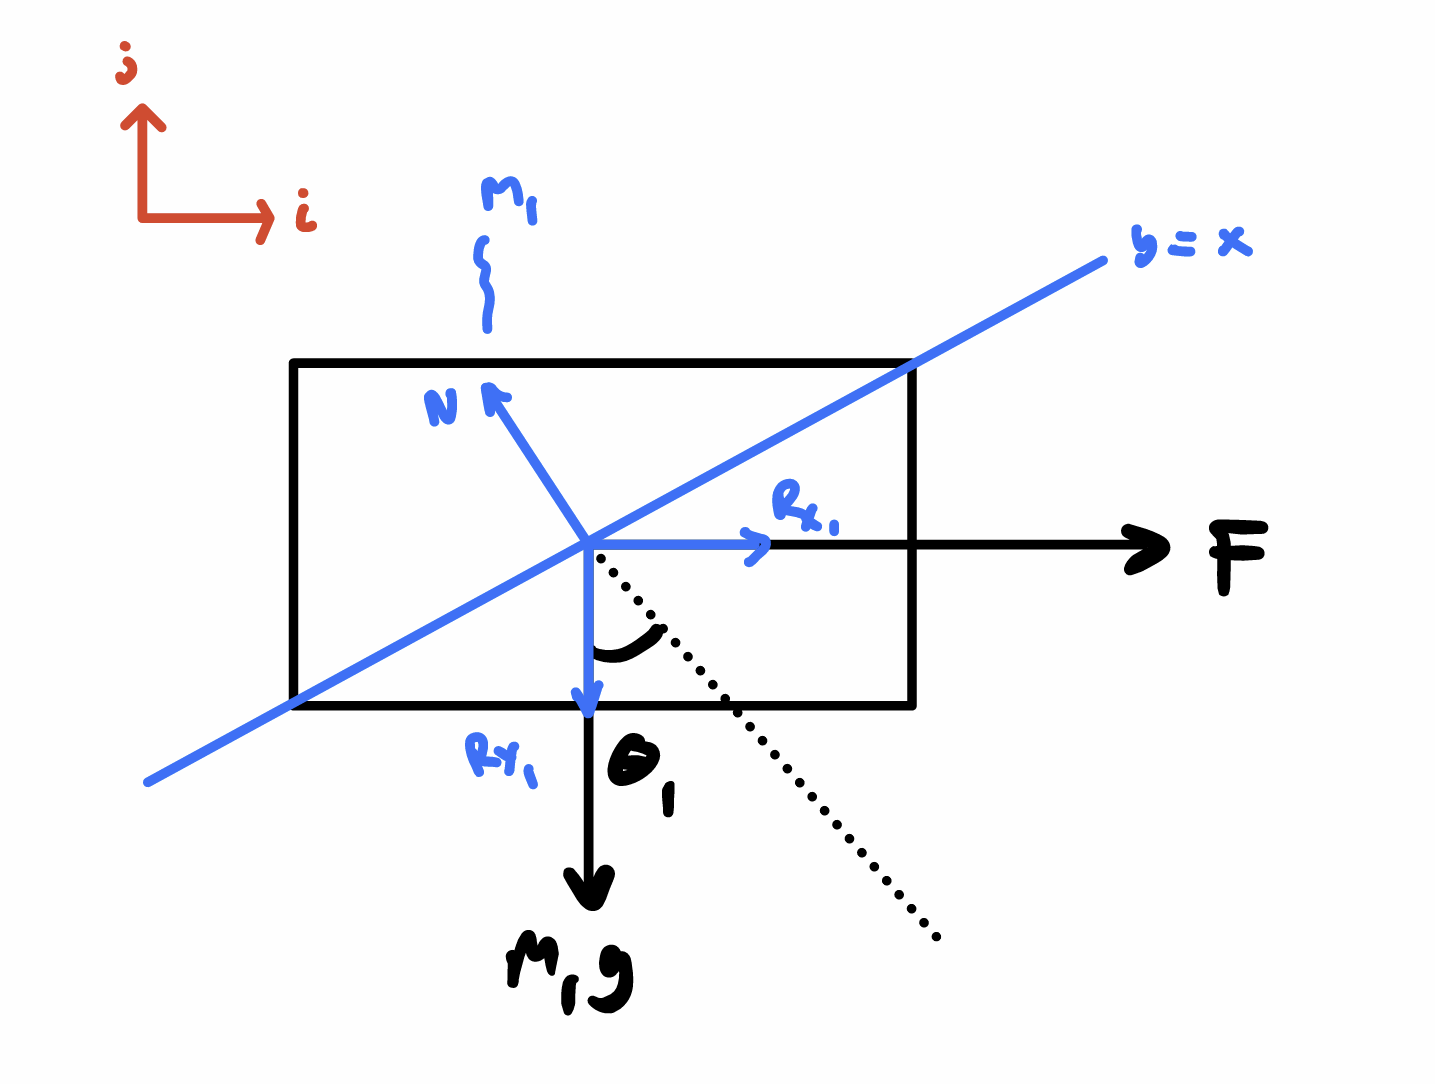
\includegraphics[width=5cm]{DAE_FBD_0} }}%
	\qquad
	\subfloat[\centering Link 1 FBD]{{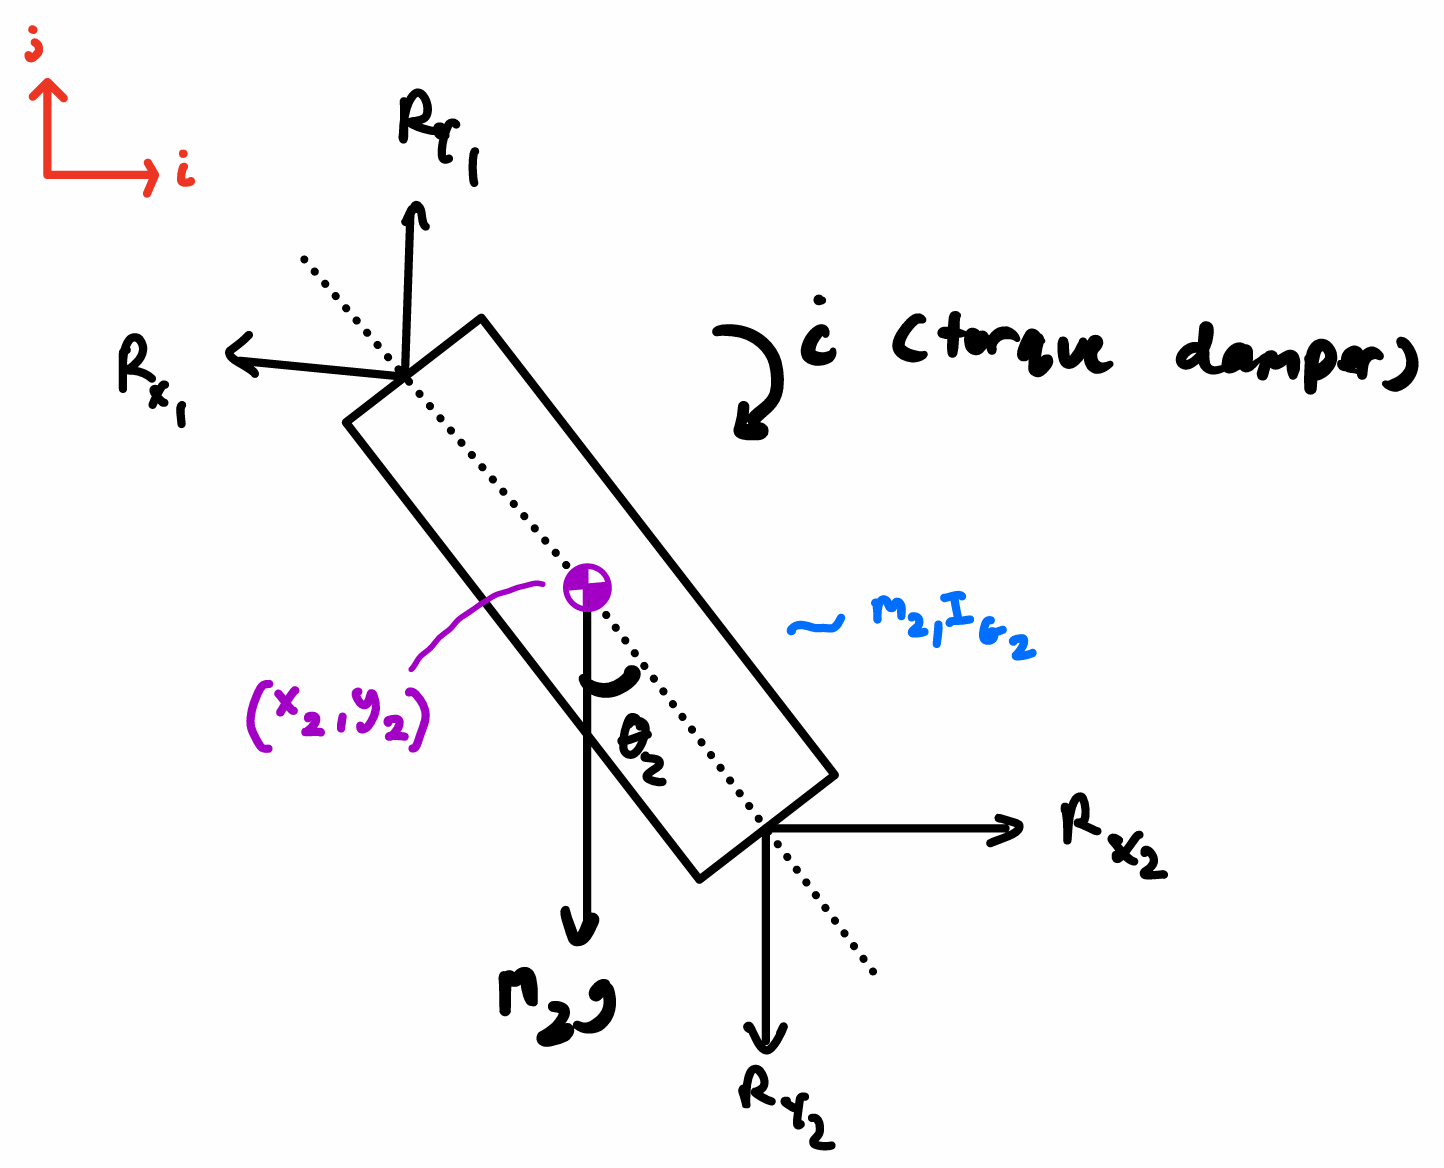
\includegraphics[width=5cm]{DAE_FBD_1} }}%\\
	\qquad
	\subfloat[\centering Link 2 FBD]{{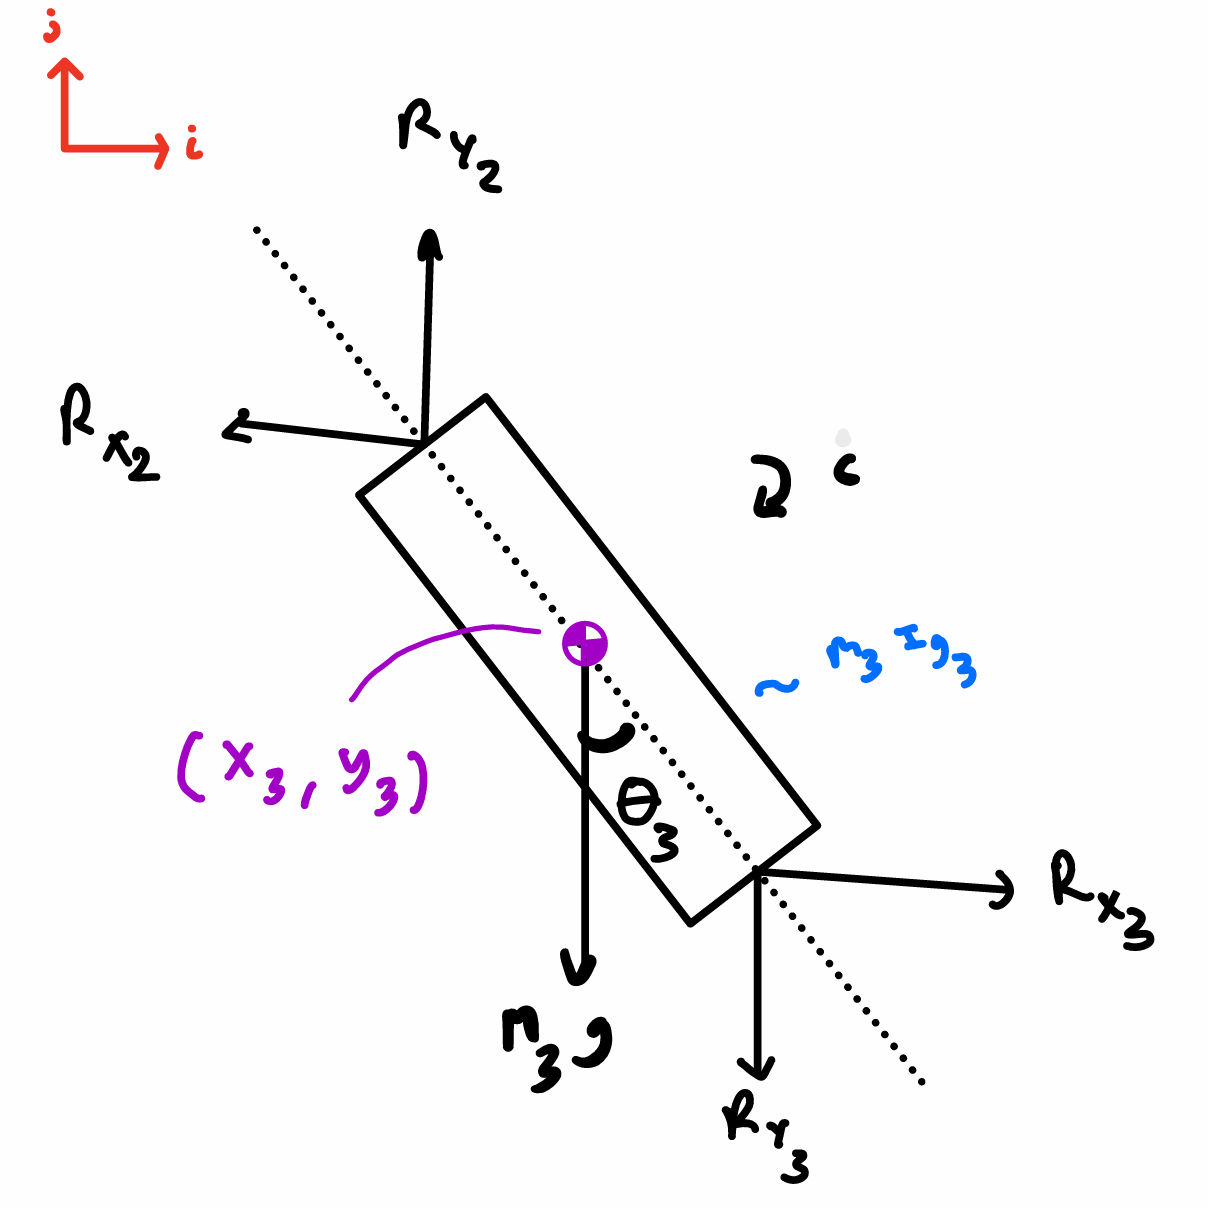
\includegraphics[width=5cm]{DAE_FBD_2} }}%\\
	\qquad
	\subfloat[\centering Link 3 FBD]{{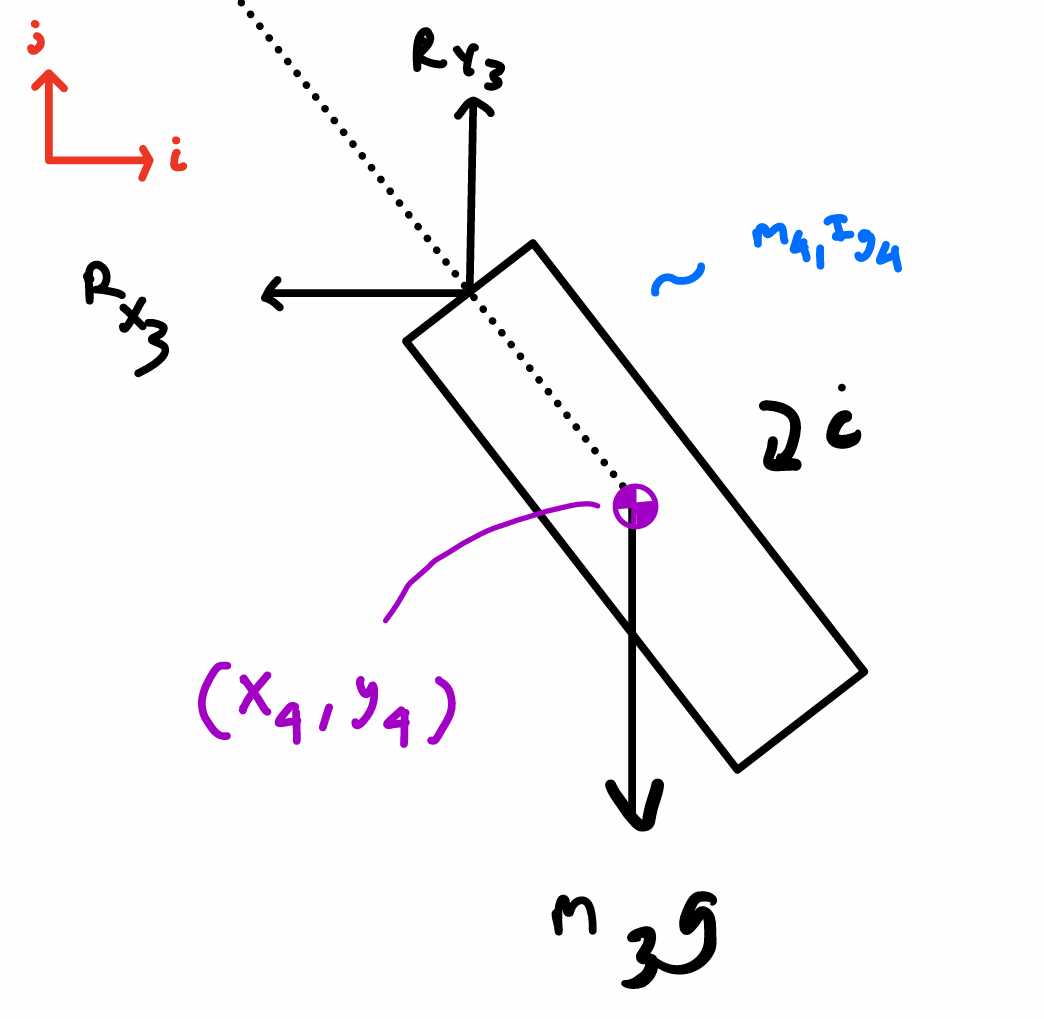
\includegraphics[width=5cm]{DAE_FBD_3} }}%\\
	\caption{Description of FBD model components}%
	\label{fig:example2}%
\end{figure}
\subsubsection{Equations}
From the free body diagrams and the DAE approach, a maximal coordinates approach is used with variables:
\begin{center}
	\begin{equation}
		q=\{x_1,y_1,x_2,y_2,\theta_1,x_3,y_3,\theta_2,x_4,y_4,\theta_3,R_{x_1},R_{y_1},R_{x_2},R_{y_2},R_{x_3},R_{y_3},F_{N_x}, F_{N_y} \}
	\end{equation} 
\end{center}
This leads to 19 unknowns, consistent with the number of equations listed above.
2

\begin{center}
	\begin{tabular}{c|c|c}
		n&Equation Origin&Equation\\
		\hline
		1&LMB in $\hat{i}$ on Sledge & $R_{x1} + F + F_{N_x} = m_1 \ddot{x}_1$\\
		2&LMB in $\hat{j}$ on Sledge & $-R_{y1} - m_1 g + F_{N_y} = m_1 \ddot{y}_1$\\
		\hline
		3&LMB in $\hat{i}$ on Link 1&$-R_{x1} + R_{x2} = m_2 \ddot{x}_2$ \\
		4&LMB in $\hat{j}$ on Link 1&$R_{y1} - R_{y2} - m_2 g = m_2 \ddot{y}_2$ \\
		5&AMB on Link 1&$R_{x1} d_1 \cos(\theta_1) - R_{y1} d_1 \sin(\theta_1) + R_{x2} d_1 \cos(\theta_1) - R_{y2} d_1 \sin(\theta_1) = I_{g1} \ddot{\theta}_1 $\\
		\hline
		6&LMB in $\hat{i}$ on Link 2&$-R_{x2} + R_{x3} = m_3 \ddot{x}_3$ \\
		7&LMB in $\hat{j}$ on Link 2&$R_{y2} - R_{y3} - m_3 g = m_3 \ddot{y}_3$ \\
		8&AMB on Link 1&$R_{x2} d_2 \cos(\theta_2) - R_{y2} d_2 \sin(\theta_2) + R_{x3} d_2 \cos(\theta_2) - R_{y3} d_2 \sin(\theta_2) = I_{g2} \ddot{\theta}_2 $\\
		\hline
		9&LMB in $\hat{i}$ on Link 2&$ -R_{x3} = m_4 \ddot{x}_4$ \\
		10&LMB in $\hat{j}$ on Link 2&$R_{y3} - m_4 g = m_4 \ddot{y}_4$ \\
		11&AMB on Link 1&$R_{x3} d_3 \cos(\theta_3) - R_{y3} d_3 \sin(\theta_3) = I_{g3} \ddot{\theta}_3$\\
		\hline
		12&Constraint for $\hat{i}$ in link 1&$x_2 = x_1(t) + d_1 \sin(\theta_1(t))$\\
		13&Constraint for $\hat{j}$ in link 1&$y_2 = y_1(t) - d_1 \cos(\theta_1(t))$\\
		14&Constraint for $\hat{i}$ in link 2&$x_3 = x_1(t) + 2 d_1 \sin(\theta_1(t)) + d_2 \sin(\theta_2(t))$\\
		15&Constraint for $\hat{j}$ in link 2&$y_3 = y_1(t) - 2 d_1 \cos(\theta_1(t)) - d_2 \cos(\theta_2(t))$\\
		16&Constraint for $\hat{i}$ in link 3&$x_4 = x_1(t) + 2 d_1 \sin(\theta_1(t)) + 2 d_2 \sin(\theta_2(t)) + d_3 \sin(\theta_3(t))$\\
		17&Constraint for $\hat{j}$ in link 3&$y_4 = y_1(t) - 2 d_1 \cos(\theta_1(t)) - 2 d_2 \cos(\theta_2(t)) - d_3 \cos(\theta_3(t))$
	\end{tabular}
\end{center}
The last two equations depend on the stage of the course and varies between the courses functions. The constraint is developed from the normal force acting on the sledge with equation $F_{N_x} + F_{N_y}\frac{dy}{dx}=0$. The second constraint comes from the double derivative of the function putting a constraint linking $\ddot{y}$ and $\ddot{x}$. The course functions and their constraints are listed below
\begin{center}
	\begin{tabular}{c|c|c}
		Function&Constraint 1&Constraint 2\\
		\hline
		$(\frac{x}{10}-3)^2+1$&$F_{N_x}+(\frac{x}{50}-\frac{3}{5})F_{N_y}=0$&$\ddot{y}=\frac{\dot{x}^2}{50} + \frac{\left(\frac{x}{10} - 3\right) \ddot{x}}{5}$\\
		$\frac{-1}{10}+16$&$F_{N_x}-\frac{F_{N_y}}{10}=0$&$\ddot{y}=\frac{-1}{10}\ddot{x}$\\
		$-(\frac{x}{10}-12)^2+10$&$F_{N_x}+(\frac{12}{5}-\frac{x}{50})F_{N_y}=0$&$\ddot{y}=-\frac{\dot{x}^2}{50}-\frac{\frac{x}{10}-12}{5}\ddot{x}$\\
	\end{tabular}
\end{center}

\section{Still Frames and Trajectory Plots}

\end{document}  